\documentclass{article}
\usepackage[pdftex]{graphicx}
\usepackage[export]{adjustbox}
\usepackage{amsmath}
\usepackage{amssymb}
\usepackage[dutch]{babel}
\usepackage{fullpage}
\usepackage{epsfig}
\usepackage[T1]{fontenc}
\usepackage{epstopdf}
\usepackage{relsize}
\newcommand{\zv}{\blacksquare}
\newcommand{\wv}{\square}
\newcommand{\R}{\mathbb{R}}
\newcommand{\N}{\mathbb{N}}
\usepackage{float}
\usepackage[caption = false]{subfig}
\usepackage{graphicx}
\usepackage{tikz}
\usetikzlibrary{matrix}
\begin{document}

\title{Elliptische Kromme Diffie-Hellman}

\author{R.L. Neuteboom (4006712) S.E.M.P. Franssen()\\
\small Universiteit Utrecht \normalsize}

\date{\today}
\maketitle
\section{Inleiding}
Tegenwoordig is het steeds belangrijker communicatie via het internet te versleutelen. Zelfs als informatie nietszeggend blijkt te zijn kunnen mensen die het onderscheppen veel daaruit opmaken. Voorbeeld hiervan heb ik gezien bij een gastcollege van het vak Databases, hier liet de gastspreker zien dat je op basis van geringe informatie over een persoon, vaak relatief eenvoudig een kleine groep mensen kan construeren die het zou kunnen zijn. Zover ik weet is het ook volledig legaal om die informatie af te tappen als het onversleuteld is.\\
Dit verslag gaat over hoe je het Diffie-Hellman protocol kunt gebruiken om versleutelde communicatie op te zetten. Voor dit protocol is een systeem nodig om in te werken. Het systeem dat we gebruiken zullen we doen met een eindige cyclische multiplicatieve groep, deze cre\"eren we met behulp van een elliptische kromme. Verder willen we het bericht ondertekenen, dit zodat de ontvanger weet dat het van ons komt, het kan namelijk zo zijn dat iemand anders contact probeert te zoeken met de ontvanger en valse berichten stuurt. Om af te sluiten gaan we in op hoe we deze technieken/algoritmen hebben ge\"implementeerd in python.
\section{Diffie-Hellman protocol}
Het Diffie-Hellman protocol is een protocol om een sleutel af te spreken die vervolgens gebruikt kan worden voor versleutelde communicatie. Het protocol berust op het feit dat een bepaalde bewerking, bijvoorbeeld multiplicatie in een bepaalde groep, niet makkelijk om te keren is.\\
Laten we het protocol beschrijven:\\
In de Cryptografie is het standaard dat de bedoeling is dat een bericht van A, Alice, naar B, Bob, gaat zonder dat E, Eve, mee kan luisteren.
\begin{itemize}
\item Alice en Bob bespreken openbaar het systeem dat ze gaan gebruiken om de sleutel van latere communicatie te bepalen, in dit verslag dus een bepaalde elliptische kromme en een punt hierop
\item Alice en Bob bedenken afzonderlijk van elkaar een priv\'{e}sleutel
\item Alice en Bob gebruiken de priv\'{e}sleutel op het punt van de elliptische kromme en sturen het resultaat naar elkaar op
\item Vervolgens gebruiken beide hun priv\'{e}sleutel op het ontvangen bericht, Alice en Bob hebben nu een gedeeld geheim die ze kunnen gebruiken voor versleutelde communicatie.
\end{itemize}
Naast elliptische krommen kan ook een ander medium worden gekozen, belangrijk is dat de volgorde van het toepassen van de priv\'{e}sleutels niet relevant is. Het protocol kan ook nog eens worden uitgebreid naar meer personen: elke persoon die je toevoegt moet dan de stappen hierboven doen, er moet dan meerdere malen een ronde komen van punten bewerken met versturen naar de anderen, dit op zo'n manier dat uiteindelijk voor iedereen het punt bekend is dat door alle priv\'{e}sleutels is bewerkt op de zijne na. Het gedeelde geheim is dan uiteraard het beginpunt met alle priv\'{e}sleutels daarop toegepast.\\
We gaan ervan uit dat Eve alle communicatie onderschept en precies weet wat ze aan het doen zijn, het enige van dit verhaal wat zij niet weet zijn de priv\'{e}sleutels en het gedeelde geheim.
Het is voor Eve genoeg om achter \'{e}\'{e}n van de priv\'{e}sleutels te komen, met deze kan ze namelijk achter het gedeelde geheim komen. De veiligheid van het systeem hangt dus af hoe moeilijk het is om gegeven het punt en het punt bewerkt met een van de priv\'{e}sleutels erachter te komen wat de priv\'{e}sleutel is.\\
Omdat we werken in een eindige groep waarbij er voor het omkeren van de bewerking geen algortime is, hangt de moeilijkheidsgraad van het oplossen van dat probleem af van de orde van de groep.

\section{Elliptische Krommen}
Elliptische Krommen kunnen gebruikt worden voor het Diffie-Hellman protocol, voordat we laten zien dat je dat kan gebruiken is het gepast te te bespreken wat elliptische krommen zijn.
Een elliptische kromme is een kromme die beschreven kan worden met punten $(x,y)\in\mathbb{R}^2$ die voldoen aan:
\begin{equation}
y^2 = x^3 + ax +b.
\end{equation}
Voorwaarde hierbij is dat dat de beschreven grafiek niet singulier is, de definitie van singulier hangt af van het type grafiek dat bestudeerd wordt.
Hier komt dat neer op dat de grafiek geen zelf-intersecties, aaneengesloten en we moeten met behulp van een bijectieve parametrisatie $p:\mathbb{R} \to \textbf{E}$ de curve kunnen doorlopen waarbij we overal de afgeleide kunnen bepalen en ongelijk aan nul zijn. Op zo'n grafiek zijn we vooral ge\"interesseerd in punten $(x,y)\in \mathbb{Z}^2$, we moeten daarom ook eisen dat $(a,b)\in\mathbb{Z}$. Reden hiervoor is dat we met de net besproken grafiek een eindige groep maken. We defini\"eren de groep $G$ dan op de volgende manier, een punt op de grafiek met gehele $x$ en $y$ is een element van onze groep. Het eenheidselement, aan te geven met $\infty$ is een punt dat niet op de grafiek ligt, je zou het kunnen zien als het toegevoegde punt voor one-point-compactification. De groepsoperatie '$+$' op punten $A$ en $B$ is op de volgende manier gedefinieerd: \\
je trekt een lijn door $A$ en $B$, laat $C$ het andere snijpunt met de grafiek zijn. Spiegel $C$ in de $x$-as en het resultaat is $A+B$.\\
Hier zitten uiteraard nog haken en ogen aan, hoe gaan we om met optellen met $\infty$ en is er wel altijd precies  \'{e}\'{e}n ander snijpunt? Aangezien we $\infty$ als eenheidselement hebben gedefini\'{e}erd nemen we gewoon het punt waarbij het wordt opgeteld als resultaat. Verder als de je een punt $A$ bij zijn $x$-as spiegeling optelt krijg je geen ander snijpunt, we noemen dan ook zijn $x$-as spiegeling $-A$ en nemen $A + -A=A -A=\infty$. Het enige wat nog laten zien moet worden is dat als je een andere combinatie van punten optelt dat er dus daadwerkelijk een derde snijpunt gevonden kan worden.(CANT REMEMBER SHIT, denk een van die webpagina's)
\subsection{Eindig maken}
Zoals we eerder vermeld hadden willen we een \emph{eindige} groep hebben, dat is de groep hierboven besproken zeerzeker niet of hij bevat alleen $\infty$ wat ook niet nuttig is. De manier waarop we dat doen is de waarden van $x$ en $y$ beperken tot een eindig veld, waarbij alleen gehele getallen zitten. Een eindig veld is een verzameling met daarbij een multiplicatie, additie, subtractie en divisie.\\
Een eindig veld $F$ heeft de volgende eisen:
\begin{itemize}
\item $F$ moet gesloten zijn in de multiplicatie en additie, d.w.z. als je twee elementen van $F$ optelt of vermenigvuldigt is dit weer een element van $F$.
\item er is associativiteit van optelling en vermenigvuldiging: $\forall a,b\in F$ geldt $a +(b + c)= (a + b) + c$ en $(a \cdot b) \cdot c = a \cdot (b \cdot c)$.
\item commutativiteit van optelling en vermenigvuldiging: $\forall a,b\in F$ geldt $a + b= b + a$ en $a \cdot b = b \cdot a$.
\item er zijn eenheidselementen van optelling en vermenigvuldiging: $e_+, e_*$.
\item er zijn additieve en multiplicatieve inversen: $\forall a \in F, \exists a^{-1}_+,a^{-1}_*\in F$ zodanig dat $a + a^{-1}_+=e_+$ en $a \cdot a^{-1}_* = e_*$.
\item distributiviteit van vermenigvuldiging over optelling: $\forall a,b,c \in F$ geldt $a \cdot (b + c) = (a \cdot b) + (a \cdot c)$.
\end{itemize}
Het veld waar wat we gaan gebruiken is $\mathbb{F}_p$ dit is het veld, waarbij de gehele getallen in restklassen modulo $p$ elementen zijn van het veld. Gegeven dat $p$ priem is voldoet $\mathbb{F}_p$ aan de eisen. Wat verder nog op te merken valt is dat we hieruit ook geheeltallige machtsverheffing kunnen gebruiken.

\section{Ondertekenen}
Voor het ondertekenen van de berichten gebruiken we een HMAC (Hash-based Message Authentication Code). Voor HMAC is een cryptografisch veilige hash-functie nodig, hiervoor gebruiken we SHA256. Anders dan bij gebruikelijke hashfuncties zijn deze gemaakt op zo'n manier dat het erg moeilijk is om twee inputs te vinden die dezelfde output geven, daarnaast moet de input niet te achterhalen zijn. De input die wij gebruiken is de versleutelde tekst. 
\section{Implementatie: chat applicatie}
Om een chat applicatie te maken hebben we het volgende gedaan:
We hebben een onversleutelde chatapplicatie (server en client) gekopieerd van het internet om later aan te passen, een paar klassen geschreven om met de elliptische krommen om te gaan en als laatse  een klasse om te versleutelen en ontsleutelen van de tekst met AES geschreven.\\
ruw bestandenoverzicht:\\
\begin{itemize}
\item AES.py de inhoud van dit bestand wordt gebruikt voor AES encryptie en decryptie.
\item EC.py wordt gebruikt om te defini\"eren wat een punt, curve en finite field is.
\item crypto.py is verantwoordelijk voor het toepassen van AES op de tekst en het afspreken van de keys met Diffie-Hellman.
\item tcp.py is het serverprogramma, deze gebruikt bovenstaande bestanden om een connectie op te zetten en communiceert alles van de aangesloten clients door, dit doet hij door met elk van de clients Diffie-Hellman protocol af te gaan.
\item telnet.py is de client, deze moet communiceren met de server, weergeven wat er binnenkomt en ook weergeven wat je hebt getypt.
\end{itemize}
\subsection{diepere werking}
hieronder een overzicht van de klassen, bestanden en de relaties ertussen, een gerichte pijl betekent dat waar de pijl naar wijst gebruikt wordt door waar hij vandaan komt. Vervolgens gaan we in op hoe de communicatie verloopt tussen server en clients.

\begin{center}
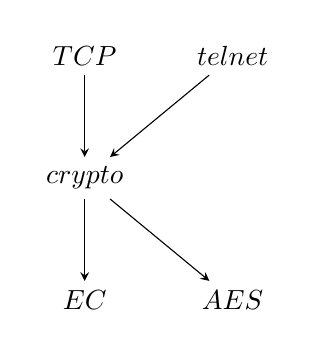
\begin{tikzpicture}
  \matrix (m) [matrix of math nodes,row sep=3em,column sep=2em,minimum width=2em]
  {
   TCP & telnet\\
   crypto \\
   EC & AES\\
   };
  \path[-stealth]

    (m-1-1) edge node [left] { } (m-2-1)
    (m-1-2) edge node [left] { } (m-2-1)
    
    (m-2-1) edge node [right] {} (m-3-1)

    (m-2-1) edge node [left] {} (m-3-2);   
\end{tikzpicture} 
\end{center}
Communicatie verloopt als volgt. Stel we verbinden als Client C met een server S. Als eerste stap zal de server alle andere gebruikers op de hoogte stellen dat er een nieuw iemand meeluisterd, ook reageert de server met de eerste stap van het DH protocoll op C. De Client stuurd zelf ook de eerste stap van het DH protocoll op. Vervolgens berekenen de Server S als de client C hun gedeeld geheim. Van dit geheim worden deelsleutels gemaakt die de up en downstream van en naar de server beveiligen. Als C een bericht wil sturen aan de anderen die verbonden zijn met de server versleuteld C zijn bericht met de upstream keys naar de server. Vervolgens verstuurd C dit bericht naar de server. De server ontvangt dit bericht en ontsleuteld deze met de upstream key van C naar de server. Nu heeft de server het bericht dat C aan alle andere clients wilde sturen. Vervolgens genereerd de server voor elke client $\tilde{C}$ een eigen versleuteling van het bericht met de downstream sleutels van $\tilde{C}$ naar de server. Vervolgens verstuurd de server dit bericht naar $\tilde{C}$. $\tilde{C}$ ontvangt dan dit bericht en kan met zijn downstream keys dit bericht ontsleutelen. 
\subsubsection{EC.py}
Dit bestand bevat alles wat nodig is om met de elliptische krommen te kunnen werken. De klasse FiniteFieldElem is ervoor om te zorgen dat er in het eindige lichaam gewerkt kan worden i.c.m. de elliptische kromme, heeft de variabele $p$ om $\mathbb{F}_p$ te kunnen vormen voor $p$ priem.\\ De klasse Curve heeft twee variabelen $a$ en $b$ zoals eerder om de kromme te defini\"{e}ren en $p$ om aan te geven op welk finitefield we werken.\\
De klasse Punt stelt een punt op een kromme voor, de variabelen x en y zijn FiniteFieldElem's, de klasse Eenheid is een subklasse van Punt en stelt het eenheidselement voor.
\subsubsection{AES.py}
Dit bestand zorgt ervoor dat tekst versleuteld kan worden d.m.v. AES. Als begin hebben we een implementatie van AES van het internet af geplukt die een blok van 16 bytes versleutelde met behulp van een 16 byte sleutel. Vervolgens hebben we deze code aangepast zodat hij een willekeurig lange stroom data kan versleuten, met behulp van codebookchaining. Deze module moet geinitialiseerd worden met een masterkey en een iv. De masterkey genereerd de rondesleutels, en deze moet elke sessie willekeurig gekozen worden of tot stand komen door een betrouwbaar key agreement protocoll, en geheim blijven. De IV hoeft alleen willekeurig te zijn. Bij een gefixeerde IV, of niet willekeurig gekozen IV daald het aantal bericht die veilig versleuteld kunnen worden zonder collisies.
\subsubsection{Crypto.py}
Dit bestand bevat de klasse LSEC, wat defini\"eert op welke kromme en eindig lichaam we werken  en de klasse crypto.
De klasse crypto gebruikt zowel AES.py als EC.py, de laatste hiervan om een sleutel af te spreken. AES om de versleuteling van de berichten te doen. Na de versleuteling worden de berichten ondertekend met een hmac gebaseerd op sha256. Er is gekozen voor encrypt then sign omdat deze methode veel minder gevoelig is voor side channel aanvallen, en dezelfde theoretische veiligheid bied. \\Verder wordt in Crypto.py verzorgd dat als er een gemeenschappelijke sleutel is afgesproken er via herhaald hashen via pbkdf2 hmac veilige sleutels en IVs worden verzorgt voor de upstream en downstream van gegevens, de IV voor die streams en de sleutels om die streams te ondertekenen met behulp van HMAC.
\subsubsection{tcp.py}
tcp.py is de python file met daarin de server code. Deze houd alle users bij met hun keys, en als er een bericht binnenkomt dan stuurd de server dit bericht door naar alle andere users van de server. De server gebruikt crypto om de berichten te versleutelen en met de clients keys af te spreken.
\subsubsection{telnet.py}
de python file telnet.py is de file die zorgt dat clients verbinding kunnen leggen met de server en kunnen communiceren. De client heeft in tegen stelling tot de server geen verbinding met alle gebruikers van de server maar alleen met de server zelf. 

\section{Aanvallen}
We bespreken in deze sectie enkele aanvalsmogelijkheden die een aanvaller hebben om het verkeer te onderscheppen. Ten eerste kan iedereen verbinding maken met de server waarop er gecommuniceerd wordt en het gesprek afluisteren. Echter, als iemand verbinding maakt wordt dit bericht naar alle andere gebruikers gepushed en zijn alle gebruikers op de hoogte dat er iemand meeluisterd. Er zijn ook andere methoden waarop de gebruikers niet op de hoogte hoeven zijn dat er iemand mee luisterd. Verder kan het protocoll gemakkelijk worden aangepast dat mensen zich moeten authenticieren via een wachtwoord voordat ze mee mogen luisteren. Dit vergt een paar kleine aanpassingen voor de communicatie zelf. Echter wordt het probleematisch om jezelf bij de server te registreren als ongeregistreerde berichten negeert worden. Hier zal een middenweg in gezocht moeten worden.
\subsection{Man in the middle}Een iemand zou zich kunnen voordoen als een betrouwbare server door al het verkeer af te luisteren. Vervolgens kan deze persoon dit verkeer door sluizen naar de echte server en tegen de server doen alsof hij de client is. Omdat ip packetten vervalst kunnen worden kan dit worden gedaan zonder dat de gebruikers er iets van merken. 
\subsection{Server omkopen}Omdat al het verkeer via de server wordt geleid en de server over alle keys beschikt, kan een kwaadwillende server al het verkeer prijsgeven. 
\subsection{Side channel aanvallen}
Onze server is niet beveiligd tegen alle sidechannel aanvallen. Onze DH suite is licht gevoelig voor timing aanvallen en die zou gebruikt kunnen worden om de interne staat van de klasse random te verraden. De klasse random is niet cryptografisch veilig en kan daarmee gegevens over de geheime sleutel van de client bemachtigen. Deze geven dan de mogelijkheid om de gedeelde sleutel te bemachtigen want met de geheime sleutel en de publieke transactie kan alles worden afgeluisterd.
\\Na de Key-Exchange zijn er geen side channel aanvalmogelijkheden bekend die van een afstand uit te voeren zijn. We gebruiken encrypt-then-sign omdat deze robuster is tegen side-channel aanvallen.
\subsection{Theoretische aanvallen}
Er bestaan ook aanvallen tegen AES en DH. Deze aanvallen zijn puur theoretisch op dit moment en zijn niet praktisch haalbaar. Als het discrete logarithme probleem wordt opgelost zou dit een flinke klap zijn voor de veiligheid van versleutingsalgorithmen gebaseerd op Diffie Helman sleutel uitwisseling. Echter zijn elliptische krommen resistanter dan andere varianten van het Diffie Helman protocoll. Verder zou het kunnen dat AES gebroken wordt en er een ciphertext aanval komt. Dit is echter onwaarschijnlijk aangezien AES een goed onderzocht protocoll is gebaseerd op wiskundig goed onderbouwde methoden. Ten derde zou men een aanval tegen bijvoorbeeld sha256 kunnen vinden zodat de message authenticatie vervalst kan worden en mensen daarna side channel aanvallen tegen gewoon cbc aes gaan doen via adaptive chosen ciphertext. Dit is echter moeilijker omdat de code die we geschreven hebben geen resultaat terug geeft over hoe lang het duurde om alles te ontsleutelen en of de ontsleuteling gelukt is. Dus via deze methode kun je ook geen delen van de data terugvinden.
\section{Conclusie}
We hebben in dit project een applicatie geschreven waarbij men redelijk veilig kan communiceren over het internet. Als een user eenmaal veilig de verbinding tot stand heeft gebracht kan men moeilijk het verkeer af luisteren. Dan is er alleen nog de optie om de server eigenaar te overtuigen de geheimen prijs te geven.
\end{document}
